\documentclass[a0,landscape]{a0poster}
\usepackage{avant}
\usepackage{graphicx}
\usepackage{multicol}
\usepackage{geometry}
\usepackage{qrcode}
\usepackage{amssymb}
\usepackage[most]{tcolorbox}
\usepackage{alltt}
\usepackage{tikz} % For custom diagrams
\usetikzlibrary{shapes.geometric, arrows.meta}

% --- Page Geometry (48x36 inches with a 1-inch margin) ---
\geometry{papersize={48in,36in}, margin=1in}

% --- Custom Box Style (Now with an empty default title) ---
\newtcolorbox{posterbox}{
    colback       = blue!5!white,
    colframe      = blue!75!black,
    breakable,
    boxsep        = 8mm,
    arc           = 5mm,
}

% --- Custom command for subsection dividers ---
\newcommand{\subsectiondivider}{\par\vspace{4mm}\centerline{\rule{0.9\linewidth}{0.4pt}}\vspace{4mm}}

\begin{document}

% === TITLE BLOCK ===
\begin{center}
    \veryHuge \textbf{A Software Tool for Planning Better Clinical Trials} \\
    \vspace{0.25cm}
    \rule{\linewidth}{1.5pt}
    \vspace{0.25cm}
    \Huge \textbf{Arnab Aich, Yuan Zhang}\\
    \huge \textit{Department of Preventive Medicine, University of Tennessee Health Science Center}
\end{center}

\vspace{0.5cm}

% === THREE-COLUMN LAYOUT START ===
\begin{multicols}{3}

% --- COLUMN 1 ---
\begin{posterbox}
    \section*{\Huge Background}
    
    \subsection*{\Large Key Questions in Clinical Trials}
    \begin{center}
        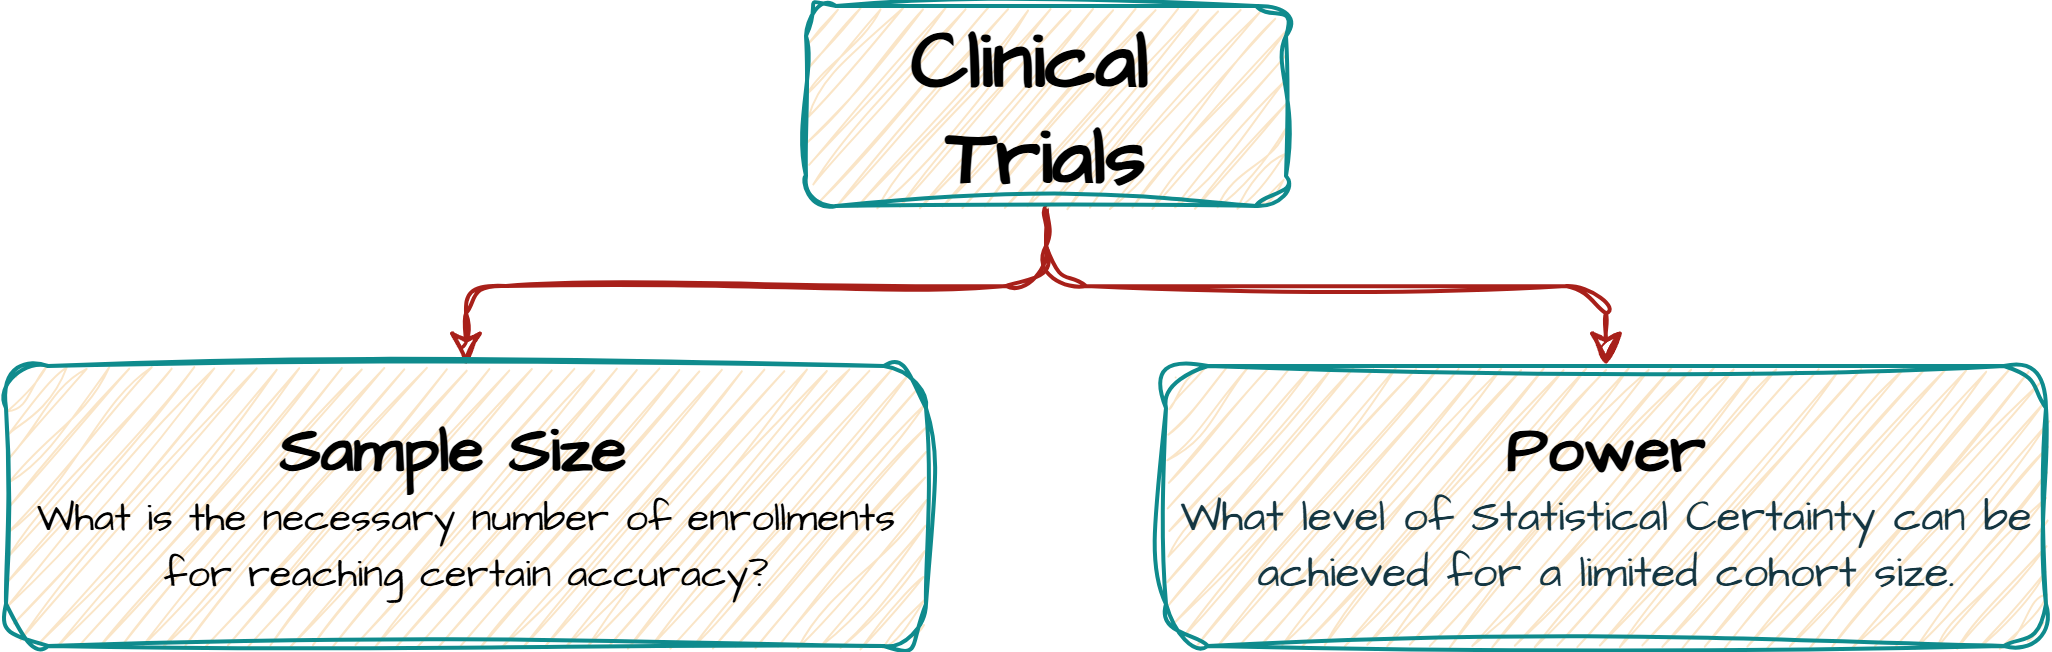
\includegraphics[width=0.8\linewidth]{images/diag-CT.png}
    \end{center}

    \subsectiondivider

    \subsection*{\Large Problems in Traditional Methods}
    \large For decades, Survival trials (\textit{Time to event}) have relied on the \textbf{HR} (Hazard Ratio).
    \begin{itemize}
        \item[\large\checkmark] This metric depends on strong assumptions that are often violated in the real world.
        \item[\large\checkmark] Can't identify treatment benefits.
    \end{itemize}

    \subsectiondivider

    \subsection*{\Large Our Solution RMST}
    \large We use \textbf{RMST} (Restricted Mean Survival Time), which directly measures the average \textbf{event-free} time patients experience.
    \begin{itemize}
        \item[\large\checkmark] It is easy for everyone to understand.
        \item[\large\checkmark] It provides a clear measure of treatment benefit.
    \end{itemize}
    \begin{center}
        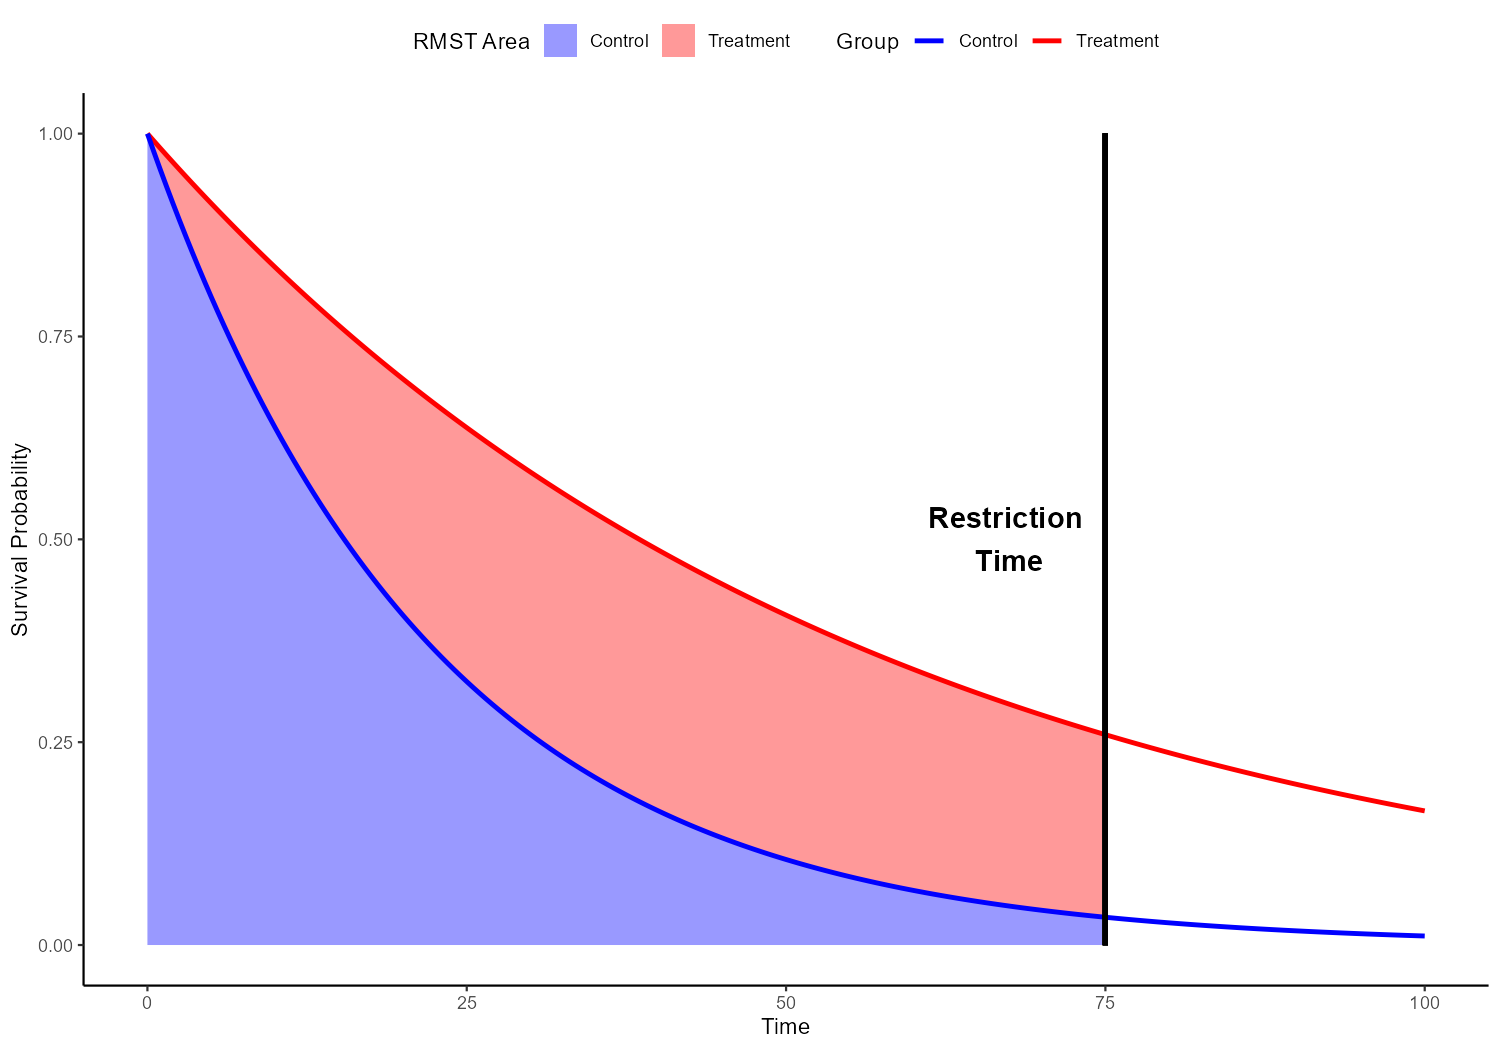
\includegraphics[width=0.8\linewidth]{images/rmst_causal_plot.png}
    \end{center}
    \large RMST difference provides causal interpretation (treatment benefits) which hazard ratios failed to provide.
\end{posterbox}

% --- COLUMN 2 ---
\begin{posterbox}
    \section*{\Huge What We Are Offering}
    
    \large ‘RMSTSS‘ is a free tool that helps researchers properly plan modern medical studies.
    \begin{center}
        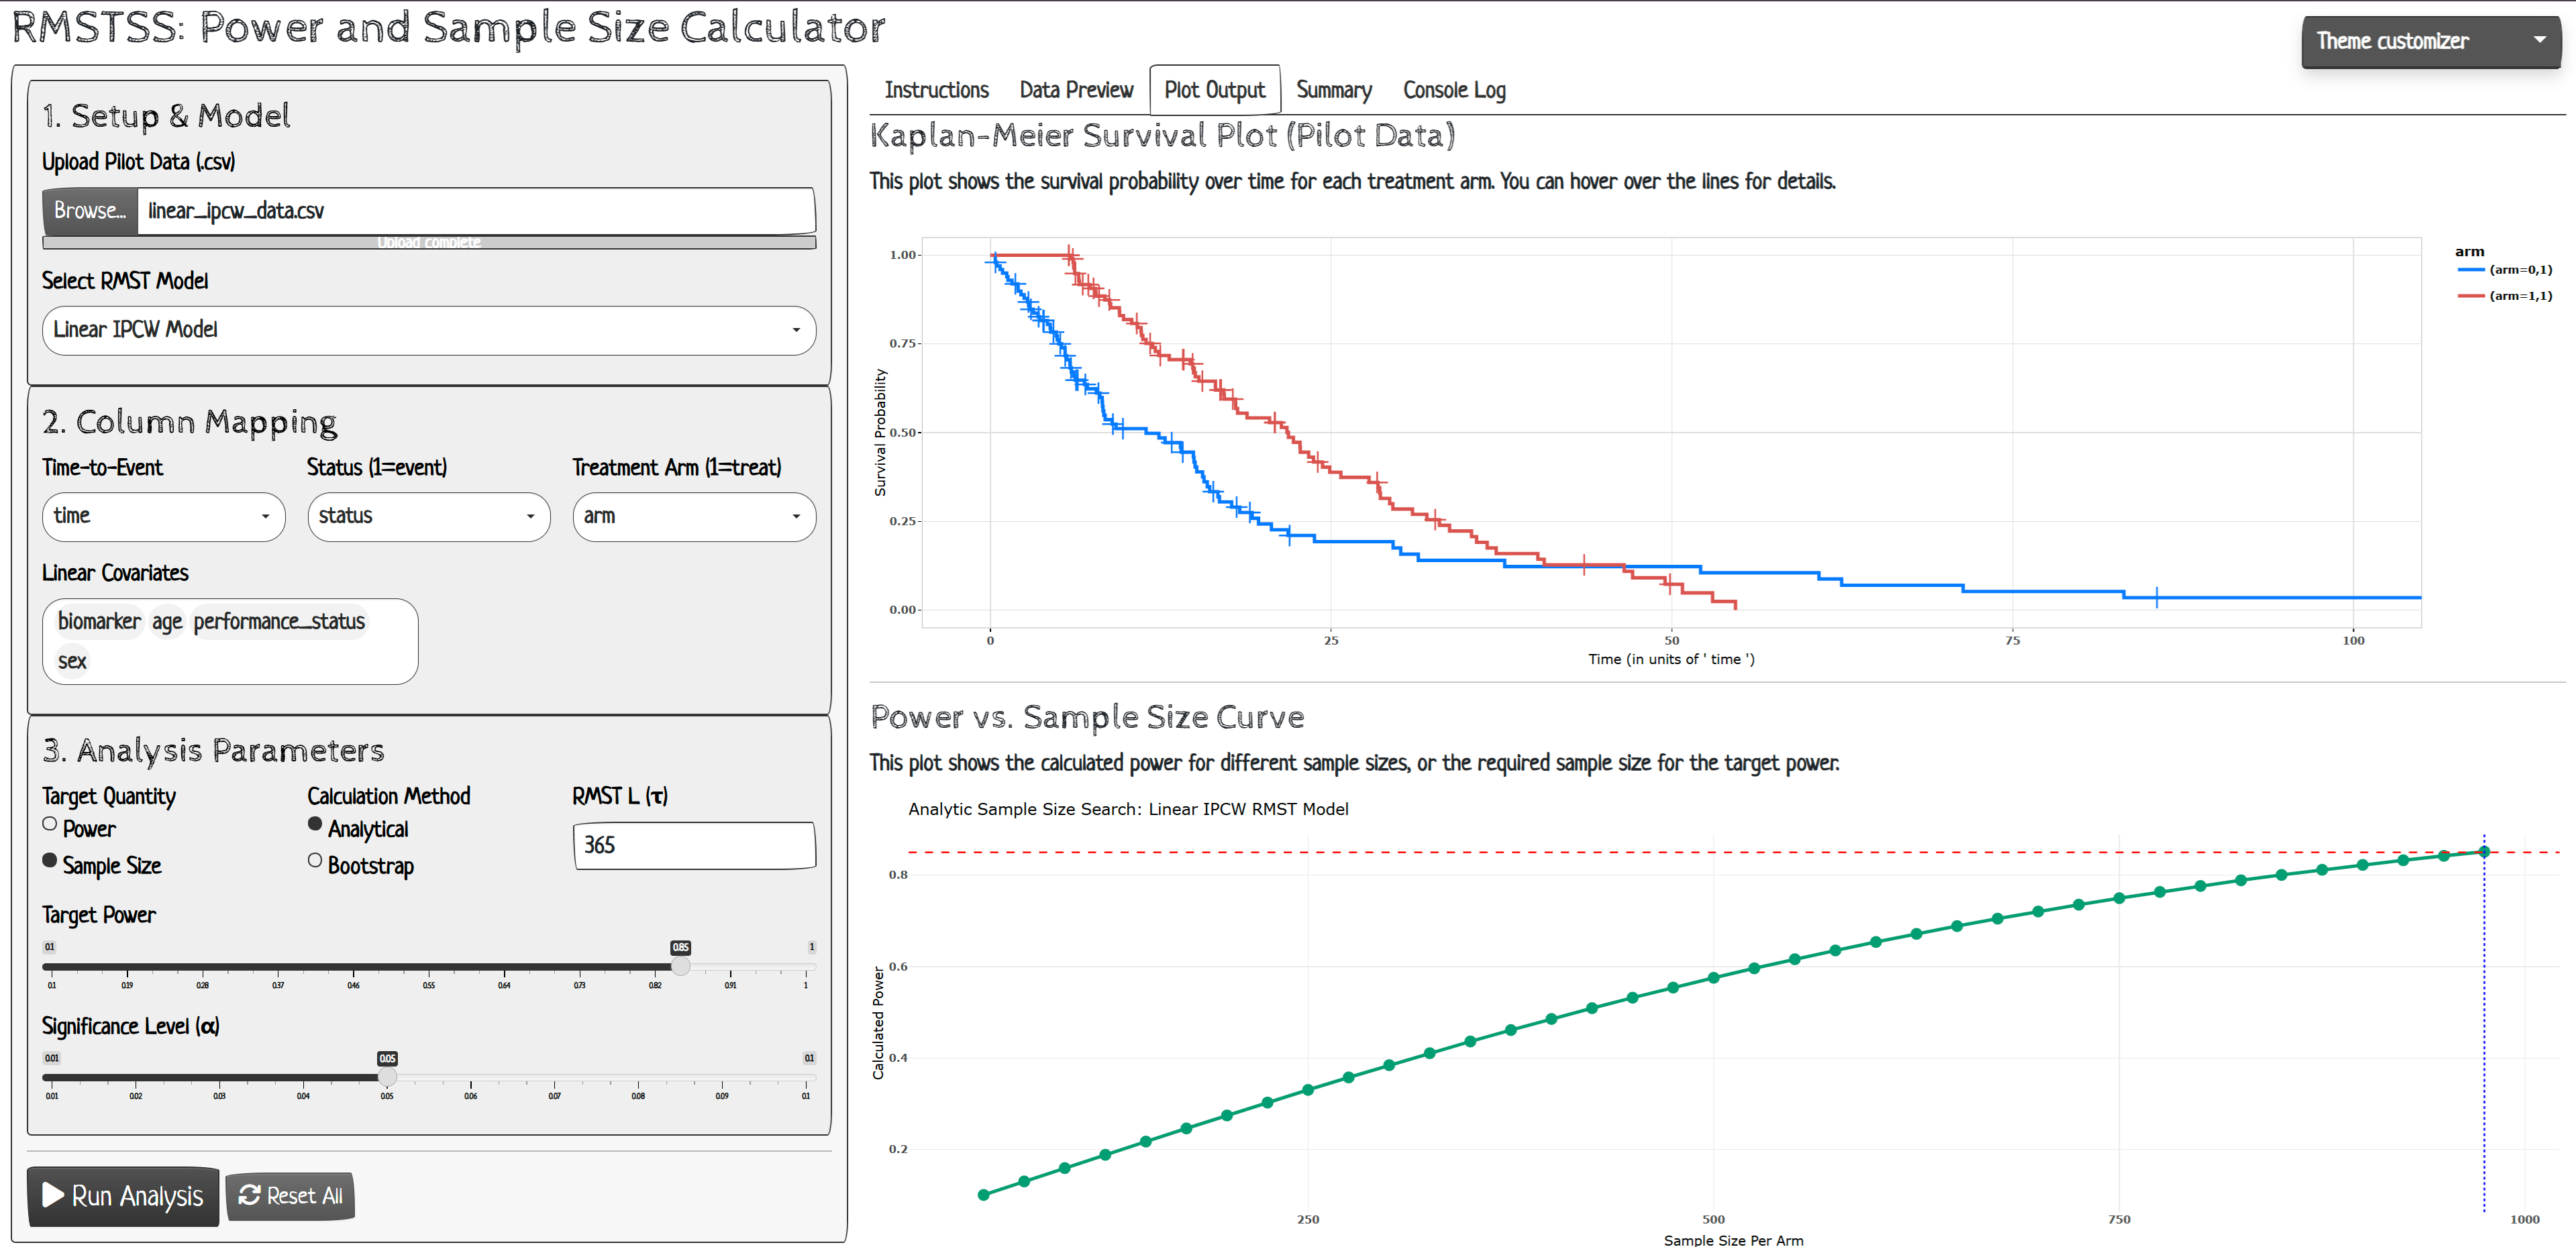
\includegraphics[width=\linewidth]{images/app-ss.png}
    \end{center}
    \large Just a glimpse of what you can do.

    \subsectiondivider
    \subsection*{\Large Available Models}
    \large Here we mention the available models which are ready to use in an instant.
    \begin{center}
        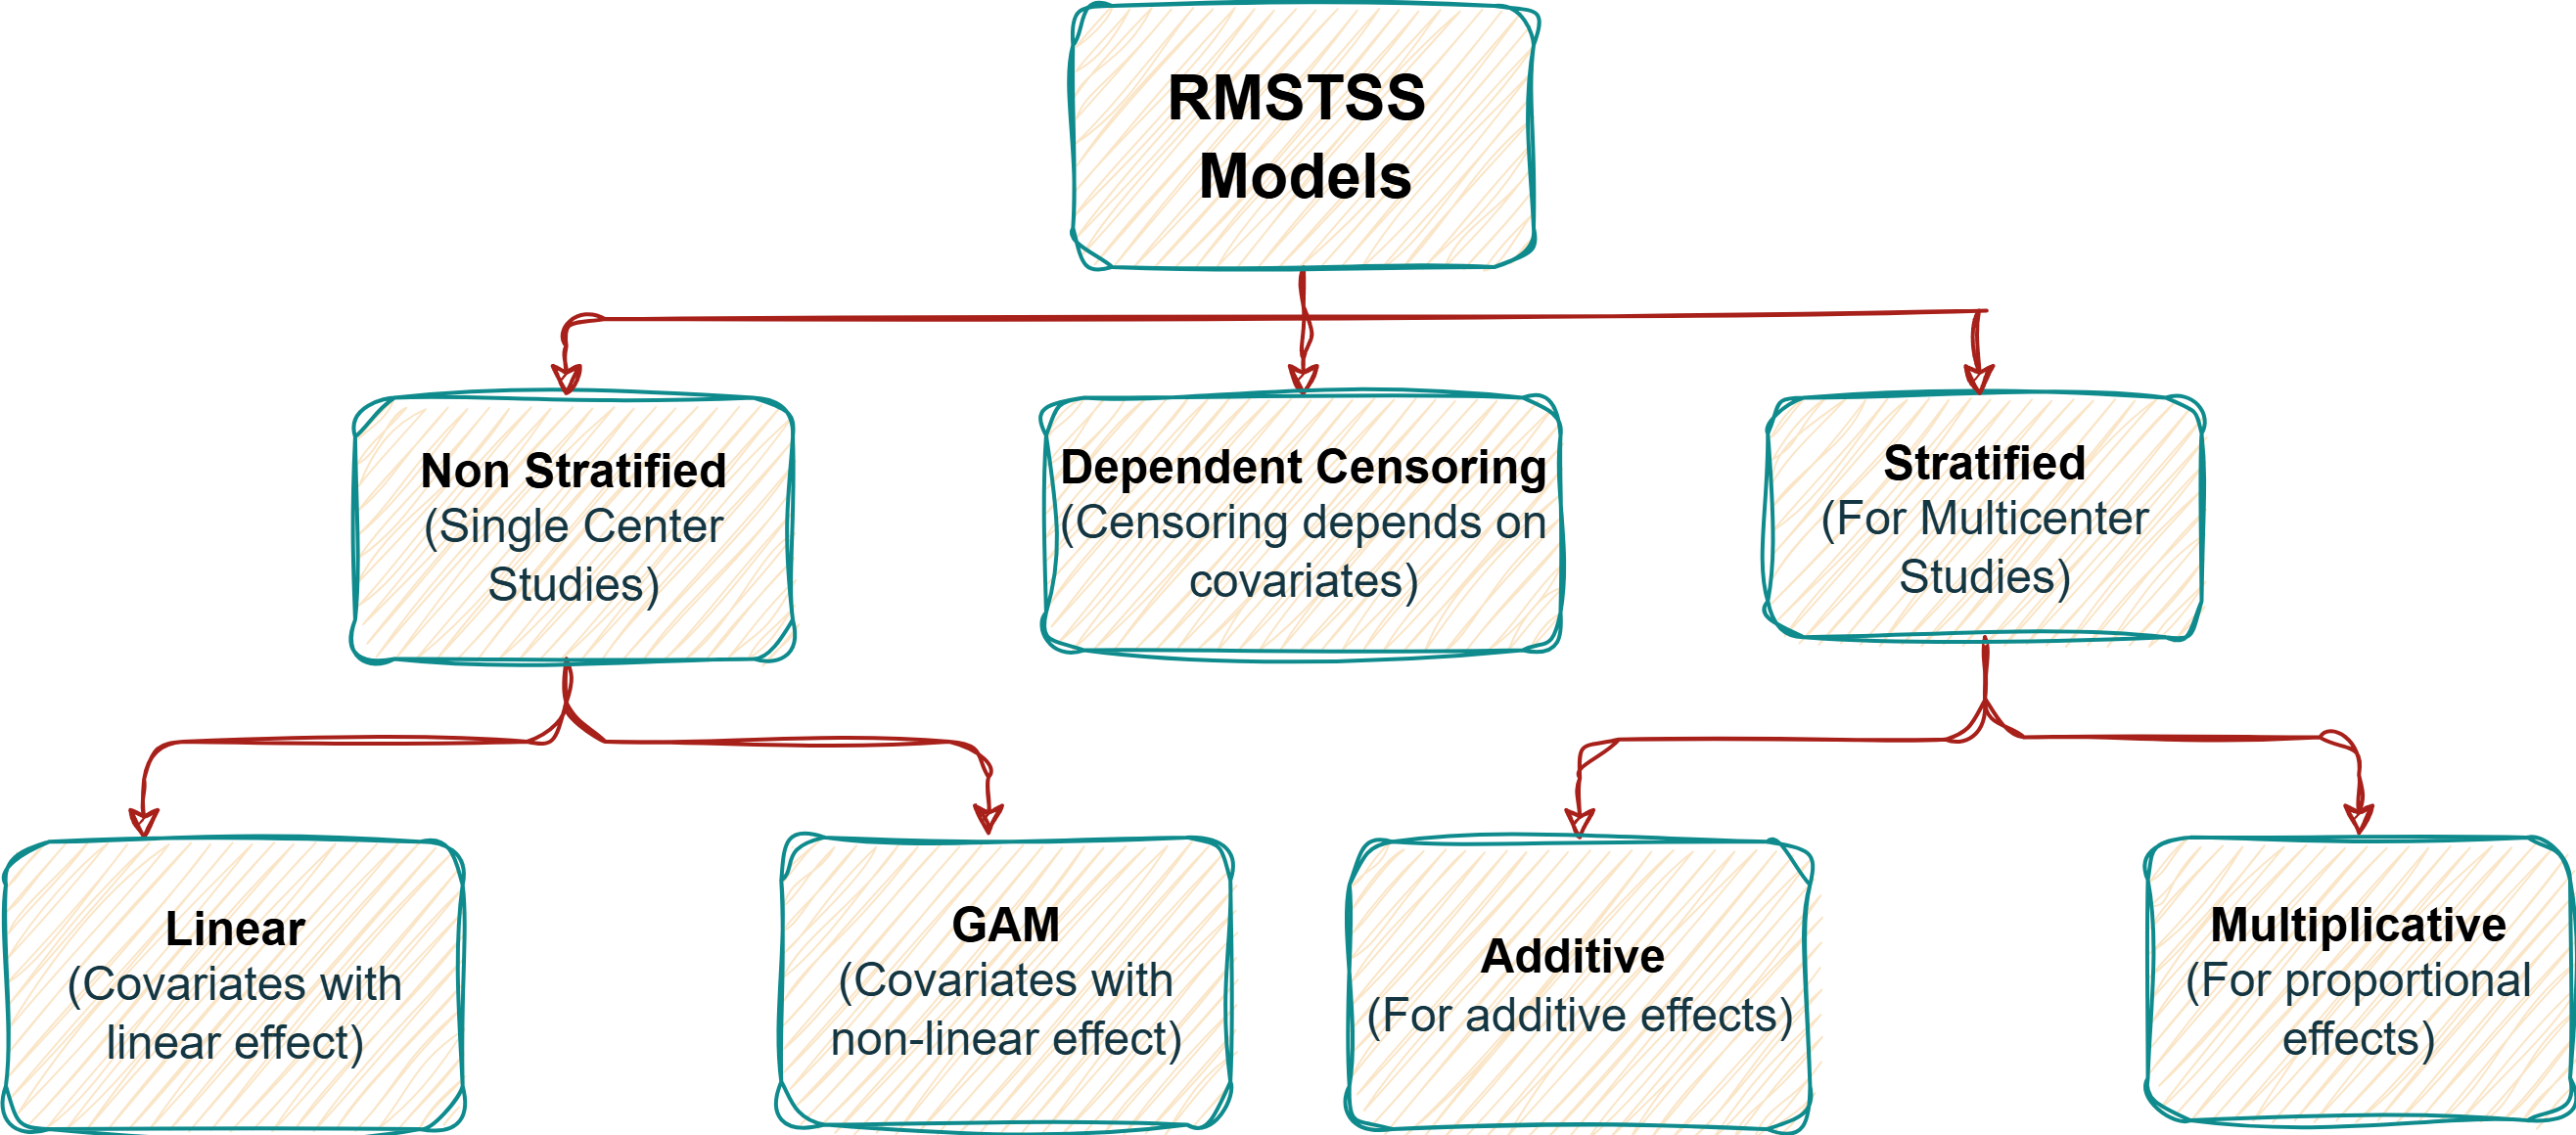
\includegraphics[width=\linewidth]{images/app-models.png}
    \end{center}


\end{posterbox}

% --- COLUMN 3 ---
\begin{posterbox}
    \subsection*{\Large App Features}
    \begin{itemize}
        \item \large \textbf{Multiple Models:} Handles standard trials, multi-hospital studies, and more.
        \item \large \textbf{Flexible Methods:} Use a \textbf{Quick Check} (Analytical) or a \textbf{Deep Dive}(Bootstrap).
        \item \large \textbf{Downloadable Reports:} Generate an HTML report for documenting purposes.
        \item \large \textbf{Customization:} Change themes, fonts, size, and many more on the go.
    \end{itemize}


    \section*{\Huge For Statisticians and Programmers}
    
    \large Besides the online app we also provide an \textbf{R-Package} for more detailed and in-depth analysis which can be downloaded from \textit{github}. It allows user to interact with the core function directly. Additionaly, after installing the package the app can be used in local machine using the following function call
    \begin{alltt}
          RMSTSS::run_app()
    \end{alltt}
    \large . For more information and project details visit the following QR-code.
    
    \begin{center}
        \qrcode[height=6cm]{https://github.com/UTHSC-Zhang/RMSTSS-Package}
    \end{center}

    \subsectiondivider
    
    \subsection*{\Large Acknowledgments}
    \begin{enumerate}
        \item NSF grant no. 2220726.
        \item UTHSC BERD (Biostatistics, Epidemiology and Research Design).
    \end{enumerate}
\end{posterbox}

\end{multicols}
% === THREE-COLUMN LAYOUT END ===

\end{document}